\documentclass[10pt,a4paper]{article} 
\fontfamily{cmss}
\usepackage{amsmath}
\usepackage{amssymb}
\usepackage{mathtools}
\usepackage[brazilian]{babel}
\usepackage[utf8]{inputenc}
\usepackage[T1]{fontenc}
\usepackage[parfill]{parskip}
\usepackage[margin=0.85in]{geometry}
\usepackage{graphicx}
\usepackage{type1ec}
\usepackage{graphicx}
\usepackage{listings}
\usepackage{hyperref}

\begin{document}

	% CABECALHO %

	\begin{minipage}[b]{0.05\linewidth}
		%\begin{figure}
			
\includegraphics[scale=0.3]{ufmg}
		%\end{figure}
	\end{minipage}
	\hfill
	\begin{minipage}[b]{0.95\linewidth}
		\begin{flushright}
			\textbf{UNIVERSIDADE FEDERAL DE MINAS GERAIS} \\
			\textsc{Graduação em Engenharia de Sistemas} \\
			\textbf{TRABALHO DE CONCLUSAO DE CURSO - PROPOSTA} \\
			Matheus Silva Araujo - 2013066265
		\end{flushright}
	\end{minipage}

	\begin{center}
		\hrulefill
	\end{center}

	% CABECALHO %
	
	\section{Introdução}
	
	O texto apresentado a seguir propõe um tema para o Trabalho de Conclusão de Curso, da graduação em Engenharia de Sistemas, UFMG.
	
	No trabalho proposto, o objetivo é apresentar uma alternativa para a representação de Modelos de Maturidade utilizando Grafos.
	
	A ideia para o trabalho é usar a disciplina Trabalho de Conclusão de Curso I para fazer pesquisa bibliográfica e modelar a solução; e na disciplina Trabalho de Conclusão de Curso II, construir uma ferramenta que utilize o modelo.
	
	\subsection{Modelos de Maturidade}
	
	Em Gestão de Projetos e Engenharia de Software, é comum a adoção de \textbf{Modelos de Maturidade}. Esses modelos visam determinar o nível de habilidade de um time ou empresa para exercer uma determinada atividade. De posse dessa informação, o time conhece suas limitações e pode traçar planos para aprimorar suas habilidades e amadurecer.
	
	Um modelo amplamente difundido no mercado é o \textit{Capability Maturity Model Integration}, CMMI. Esse modelo defende que \emph{A qualidade é influenciada pelo processo} e procura \emph{Melhorar o processo de uma empresa}.
	
	O CMMI utiliza duas representações diferentes:
	
	\begin{itemize}
	    \item \textbf{Contínua} - nessa representação os processos são avaliados de forma independente, cada um tem seu próprio nível, entre 0 e 5.
	    \item \textbf{Por Estágios} - nesse formato os processos são avaliados em conjunto, e todos devem estar no mesmo nível ao mesmo tempo, pois um nível é base para o próximo.
	\end{itemize}
	
	\subsection{\emph{DevOps} e Maturidade}
	\label{introducao_devops_maturidade}
	
	No universo do Desenvolvimento de Software contemporâneo, o \emph{DevOps} é a combinação entre pessoas, práticas e produtos no centro de um movimento que busca garantir entregas de software mais rápidas, com menos falhas e que geram mais valor para o negócio.
	
	Também existem modelos de maturidade para DevOps, um deles é o proposto por Marco Mendes, disponível em \url{https://www.dropbox.com/s/qejh6vtnwe75la5/Arkhi-MaturidadeDevOps.pdf?dl=0}
	
	Esse modelo utiliza uma representação contínua e considera oito dimensões, com cinco diferentes níveis:
	
	\begin{itemize}
	    \item Qualidade do código
	    \item Configuração como código
	    \item Gestão de builds
	    \item Gestão de testes
	    \item Testes de carga
	    \item Gestão de configuração
	    \item Gestão de releases
	    \item Monitoração de aplicações
	\end{itemize}
	
	\section{Problema}
	
	As representações contínua e por estágio são modelos simplificados do mundo real. 
	Na representação contínua, as relações entre os diferentes processos (ou dimensões) é desconsiderada para que cada processo esteja em um nível independente. E na representação por estágios, as relações entre diferentes níveis são mantidas, no entanto a dependência entre os diferentes processos impede o avanço isolado de um processo.
	
	\section{Proposta}
	
	No trabalho, a proposta é representar os modelos de maturidade utilizando Grafos. Cada nó do grafo seria um nível de maturidade em um processo (ou dimensão). As arestas seriam as representações de dependência entre os níveis por processo.
	
	Essa representação é menos rígida do que as anteriores e permite análises que não são triviais nas representações atuais. É possível, por exemplo, calcular a quantidade de níveis-processos que são habilitados por um certo nível-processo através de algoritmos de busca em grafos, \emph{Depth-First Search} ou \emph{Breadth-First Search}
	
	\subsection{Construção do Grafo}
	
	Para a construção do Grafo, um algoritmo preliminar seria:
	
	\begin{enumerate}
	    \item Enumerar as habilidades - nível-processo
	    \item Definir as relações de dependência através de uma matriz de adjacências. Virtualmente, o grafo do modelo é um grafo direcionado completo.
	\end{enumerate}
	
	Um dos objetivos do trabalho é definir melhor esse algoritmo.
	
	\section{Objetivo e metodologia}
	
	No trabalho, pretende-se pesquisar sobre os Modelos de Maturidade e também estudar Teoria de Grafos. Unindo esses dois conhecimentos, a ideia é apresentar uma proposta de representação dinâmica e mais aderente à complexidade do mundo real.
	
	Na disciplina Trabalho de Conclusão de Curso I, pretende-se fazer o levantamento bibliográfico e construir o modelo matemático bem como um algoritmo para criação do modelo. Já na disciplina Trabalho de Conclusão de Curso II, a ideia é construir uma ferramenta que desenhe o grafo e faça cálculos sob o grafo, como a análise da quantidade de nós habilitados por um nó. A ferramenta seria baseada no Graphviz \footnote{https://graphviz.gitlab.io/}.
	
	\section{Exemplo 1 - DevOps}
	
	A Figura \ref{fig:grafo_devops} apresenta um grafo para o Modelo de Maturidade DevOps apresentado em \ref{introducao_devops_maturidade}.
	
	Nesse grafo, os nós são os diferentes níveis em cada uma das dimensões do modelo. As arestas entre eles mostram as relações de dependência.
	
	A opacidade de um nó representa se um nível-processo já foi atingido, pode ser atingido ou ainda é inalcançável. 
	
	As arestas foram definidas com base em experiências do autor, mas podem ser construídas de acordo com as experiências do próprio time que esteja seguindo o modelo de maturidade, ou de acordo com orientações da comunidade.
	
	\begin{figure}
	    \centering
	    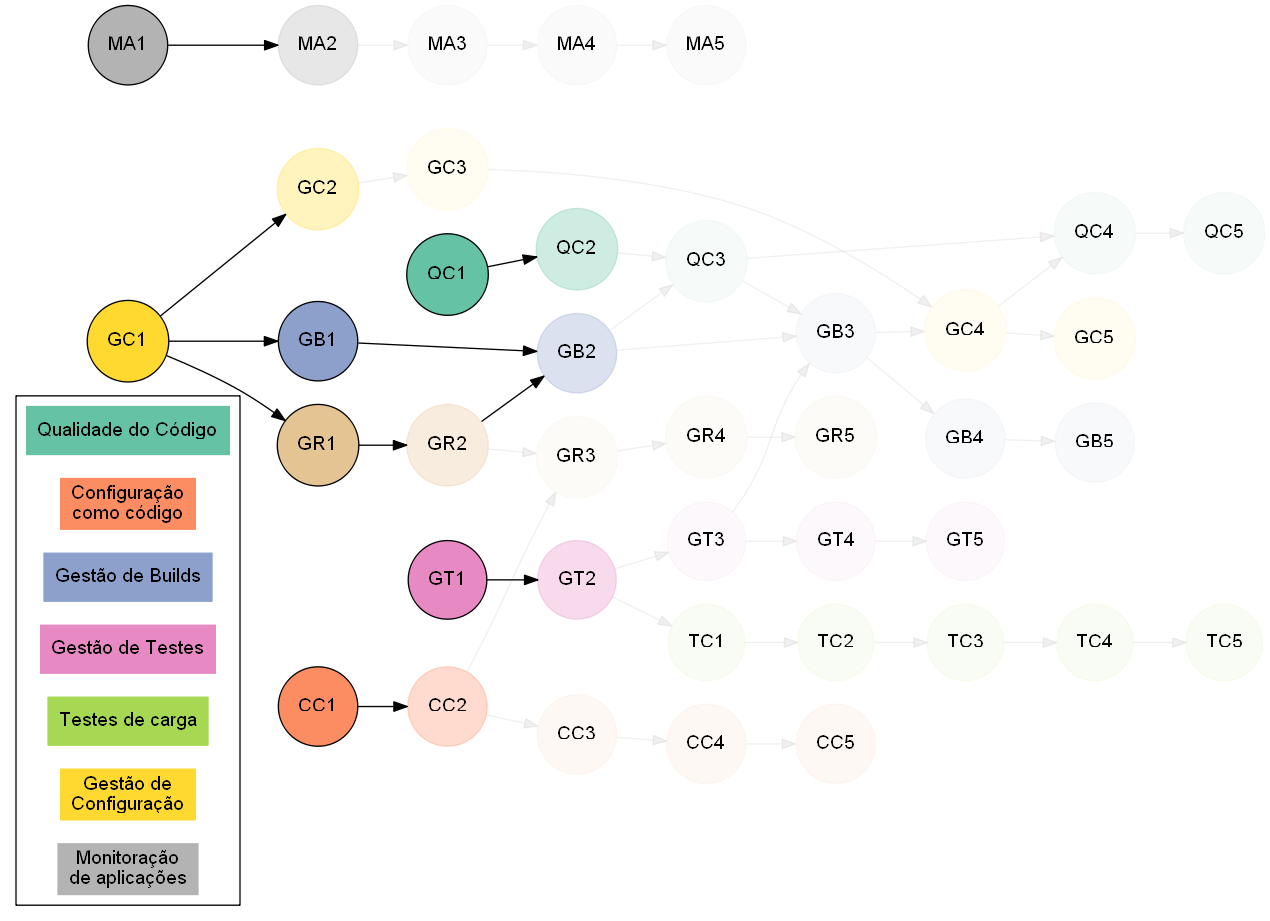
\includegraphics[width=0.8\textwidth]{grafo_devops.png}
	    \caption{Grafo para o Modelo de Maturidade DevOps}
	    \label{fig:grafo_devops}
	\end{figure}
	
	\section{Exemplo 2 - Engenharia de Sistemas}
	
	Além dos modelos de maturidade, a representação em grafos pode ser utilizada para sistemas onde existam relações de dependências não-lineares e multidimensionais, como o próprio curso de Engenharia de Sistemas.
	
	A Figura \ref{fig:grafo_engsis} apresenta um modelo de maturidade para o curso de graduação em Engenharia de Sistemas da UFMG. Cada nó representa uma disciplina, na versão curricular N-20182, as arestas são as relações de pré-requisitos formais das disciplinas. Os nós preenchidos representam as disciplinas em que o autor já foi aprovado.
	
	\begin{figure}
	    \centering
	    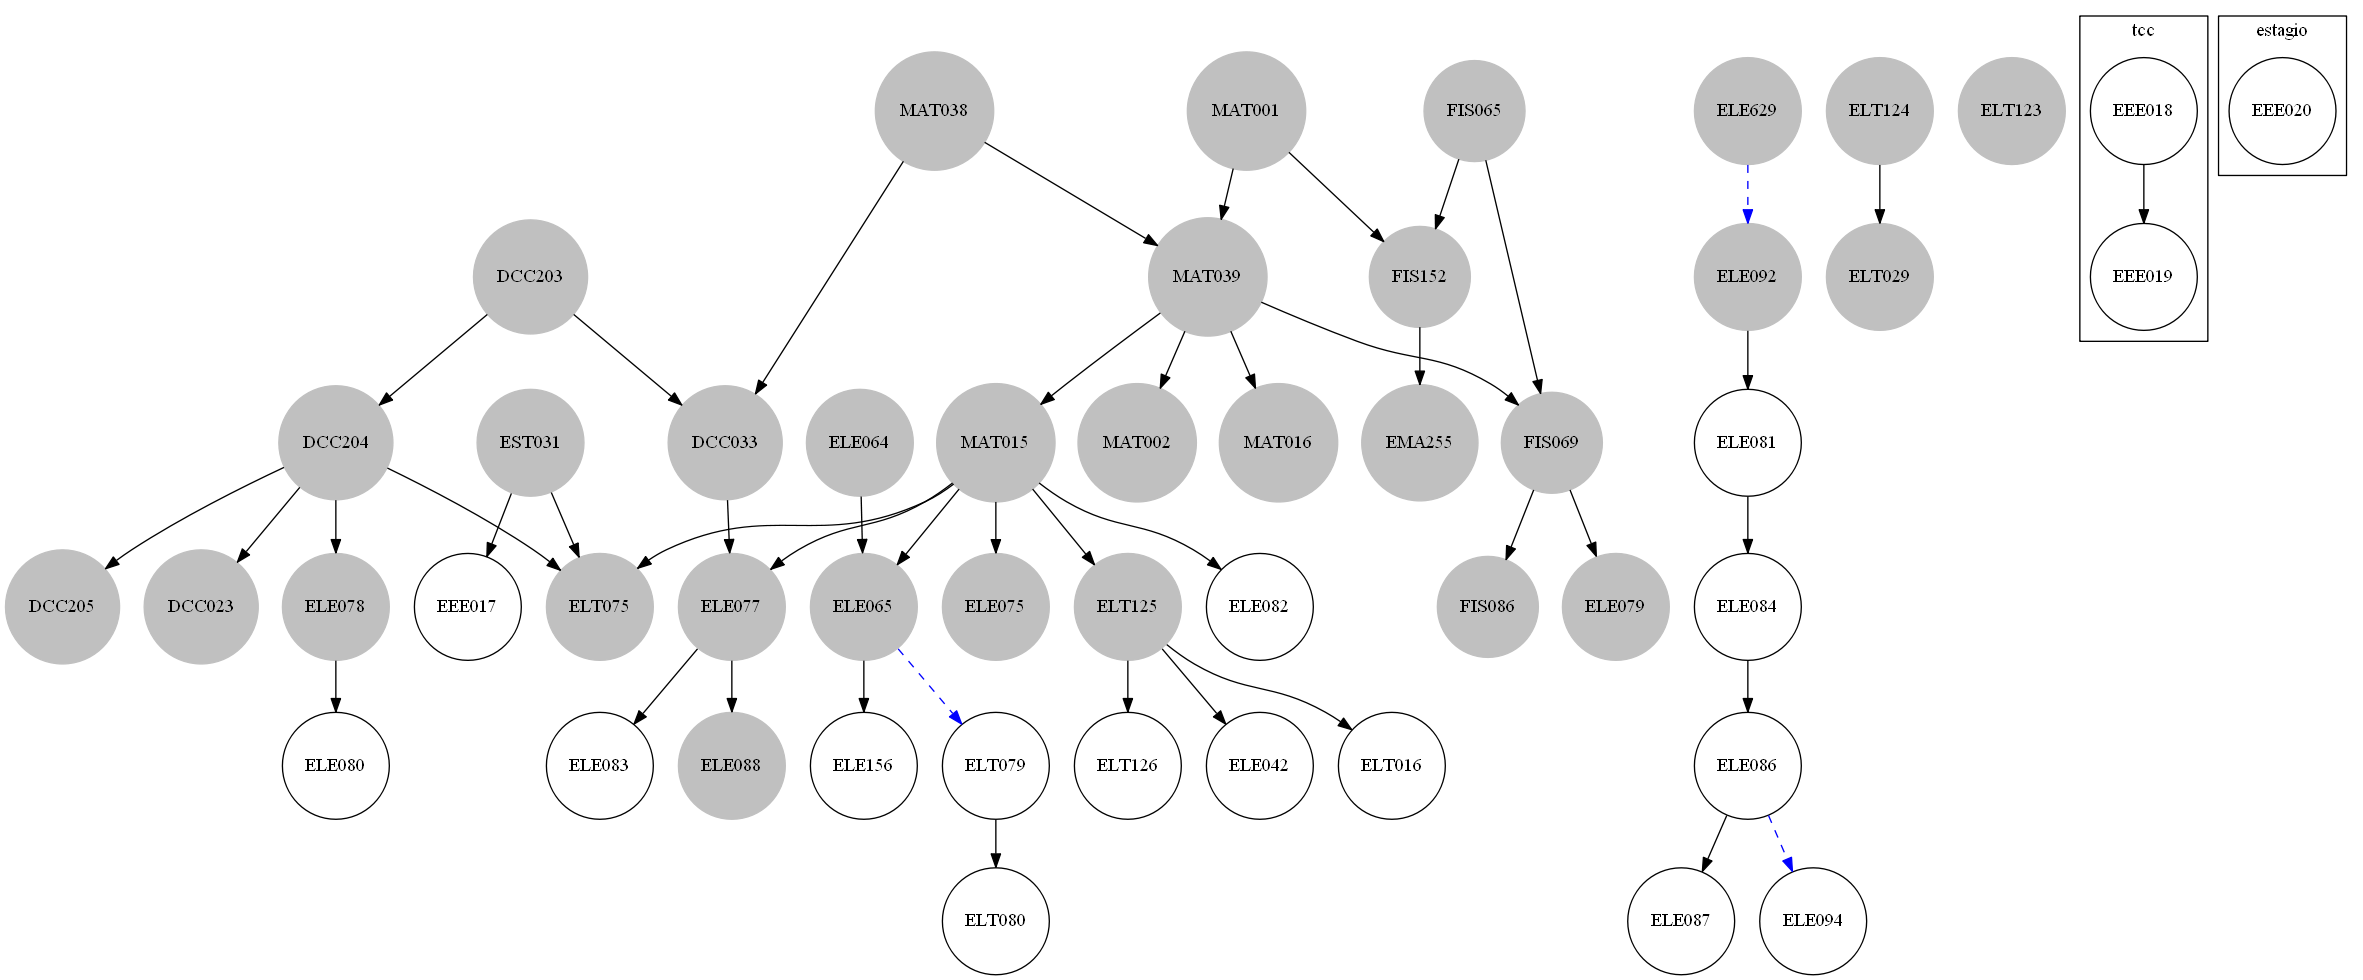
\includegraphics[width=0.8\textwidth]{grafo_engsis.png}
	    \caption{Grafo para o Curso de Engenharia de Sistemas}
	    \label{fig:grafo_engsis}
	\end{figure}

\end{document}